\chapter{Implementation}
\label{implementation}

This chapter presents the algorithm for checking composition, the implementation of activations and heaps, and I/O facilities for an interpreter designed for the \rcgo programming language presented in Chapter~\ref{language}.

\section{Interpreter Organization and Implementation}
\label{interpreter}

The interpreter consists of a scanner, a parser, a sequence of semantic checks, a code generation phase, composition checks, and an execution phase.
The interpreter is implemented in C++.
Flex and Bison were used to implement the scanner and parser, respectively.
The semantic checks include type checking and enforcement of intrinsic and indirection mutability as set forth in Chapter~\ref{language}.
The code generation phase converts the AST into a tree of stack operations.
The composition check synthesizes transactions and checks them for soundness (Section~\ref{sound_composition}).
The execution phase begins by initializing component instances by calling the initializer associated with each instance.
The scheduler then proceeds by executing transactions according to the fairness criteria of Chapter~\ref{scheduler}.
The scheduler implementations use the POSIX threads (pthreads) library for concurrent execution and synchronization.
The code is available on GitHub\footnote{\href{https://github.com/jrw972/rcgo}{https://github.com/jrw972/rcgo}}.

\section{Enforcing Sound Composition}
\label{sound_composition}

This section outlines the algorithm for checking the composition semantics of reactive components.
As described in Chapter~\ref{model}, one of the goals for the reactive component model is to facilitate the construction of complex reactive systems through composition.
The composition semantics of reactive components overcome limitations of I/O Automata and UNITY but introduce concurrency hazards that could result in systems whose behavior is not well defined.
Two key hazards to be avoided are non-deterministic transactions arising from the same state being updated by multiple transitions within a transaction, and recursive transactions arising from cycles in composition.
The goal of the composition check is to determine whether a system is free of these hazards.

Checking for sound composition is a holistic problem.
Ports facilitate third-party composition by being opaque, meaning that the action or reaction activating a port cannot know about the state transitions executed as a result of activating the port.
The state involved in a transaction is not known until the components are instantiated and the ports bound.
Thus, checking for sound composition requires a reasonably complete understanding of the system.
To this end, the algorithm described in this section leverages the static system assumption\footnote{I.e., that all components are known \emph{a priori} and no components are added or removed from the system at runtime.}.
We leave relaxing the static system assumption, which will require extending the model and proposed checking algorithm, to future work.

The reactive component semantics introduced Chapter~\ref{model} entail a number of assumptions that allow composition checking to be formulated as a set of simple graph- and set-theoretic problems.
Activate statements are limited to the bodies of actions and reactions, and port calls are limited to activate statements.
Activate statements terminate the execution of an action or reaction, meaning at most one activate statement will be called per action or reaction body.
Thus, a transaction can be viewed as a directed graph where each node is an action or reaction and edges indicate that the source action or reaction activates the target reaction.
With this graph in place, the state involved in a transaction can be deduced by treating the component instances as proxies for their state variables by creating sets of instances and evaluating the sets for compatibility.

The checking algorithm consists of several distinct steps, each of which is described next in further detail.
These steps are performed in the order they are presented as later steps depend on earlier ones.

\paragraph{Enumerate instances and ports.}
The first step to checking composition is to enumerate the components in the system using the static system assumption.
The top-level components are given by the declared instances.
Sub-components are enumerated by recursively instantiating fields that are also components.
Let $I$ denote the set of component instances.
Fields that are ports are also enumerated.
Let $S$ denote the set of push ports and $L$ denote the set of pull ports.

\paragraph{Enumerate bindings.}
Let $i$ be a component instance of type $c$.
Associated with $c$ is a set of binders $B$.
Each binder $b \in B$ is evaluated for $i$ to create a set of bindings.
A binding either binds a push port to a reaction or a getter to a pull port.
Let $R$ denote the set of reactions and $G$ denote the set of getters.
The result of enumerating the bindings is two functions (look-up tables).
The function $\mathit{reactions}: S \to \{ R \}$ maps a push port to a set of reactions.
The function $\mathit{getters}: L \to \{ G \}$ maps a pull port to a set of getters.

\paragraph{Check bindings.}
Inverting $\mathit{reactions}$ yields a function that maps a reaction to a set of push ports, $\mathit{reactions}^{-1}: R \to \{ S \}$.
The $\mathit{reactions}^{-1}$ function is used to ensure that a reaction either is bound to one push port or is not bound:
\begin{equation}
\forall r \in R : |\mathit{reactions}^{-1} (r)| \leq 1
\end{equation}
The $\mathit{getters}$ function is used to ensure that a pull port is bound to exactly one getter:
\begin{equation}
\forall l \in L : |\mathit{getters} (l)| = 1
\end{equation}

\paragraph{Enumerate transactions.}
Let $i$ be a component instance of type $c$.
Associated with $c$ is a set of actions $A$.
Each action $a \in A$ is evaluated for $i$ to create a transaction.
A \emph{transaction} is a directed graph constructed as follows, as the example in Figure~\ref{transaction} illustrates:
\begin{enumerate}
\item The root is an action $a$.
\item The descendants of the root are the activations in $a$ and the pull ports and the getters used in the immutable phase.
\item The descendants of the pull ports are the getters bound to the pull ports given by $\mathit{getters}$.
\item The descendants of the activations are the push ports named in each activation.
\item The descendants of the push ports are the reactions bound to the push ports given by $\mathit{reactions}$.
\item This process is then repeated for each reaction and getter.
\end{enumerate}

\begin{figure}
\centering
%%\resizebox{\textwidth}{!}{%
\begingroup
\fontsize{10pt}{12pt}\selectfont
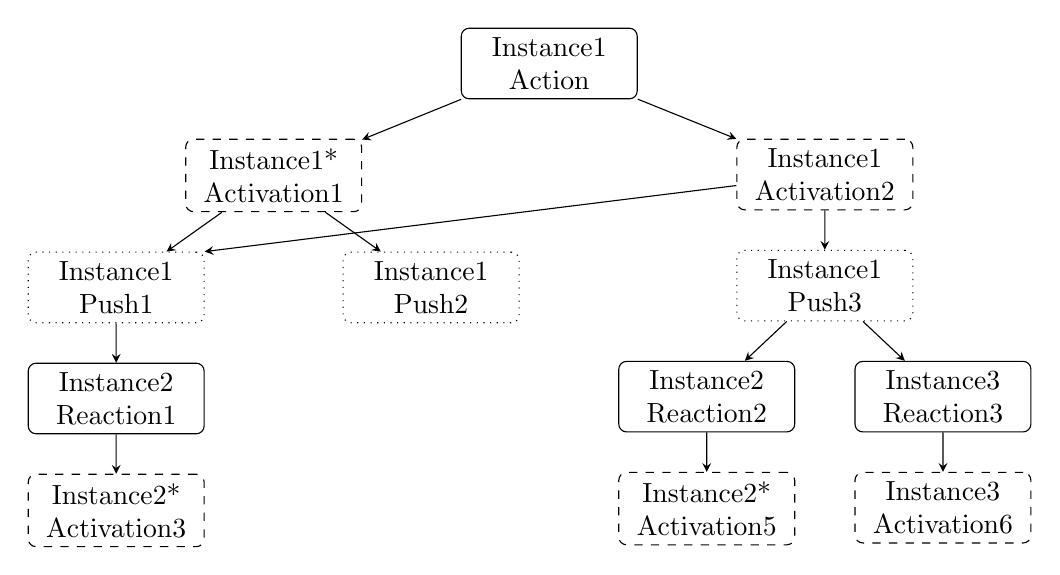
\begin{tikzpicture}[
    arrowstyle/.style={draw, -stealth},
    edge from parent/.style={draw, -stealth},
    reaction/.style={rectangle, draw, rounded corners=1mm, text width=2cm,
        text centered, anchor=north},
    activation/.style={rectangle, draw, rounded corners=1mm, dashed, text width=2cm,
        text centered, anchor=north},
    push/.style={rectangle, draw, rounded corners=1mm, dotted, text width=2cm,
        text centered, anchor=north},
    level 1/.style={sibling distance=7.0cm},
    level 2/.style={sibling distance=4.0cm},
    level 3/.style={sibling distance=3.0cm},
    level distance=0.5cm, growth parent anchor=south
]
\node (Action) [reaction] {Instance1 Action}
  child {
    node (Activation01) [activation] {Instance1* Activation1}
    child {
      node (Push01) [push] {Instance1 Push1}
      child {
        node (Reaction01) [reaction] {Instance2 Reaction1}
        child {
          node (Activation03) [activation] {Instance2* Activation3}
        }
      }
    }
    child {
      node (Push02) [push] {Instance1 Push2}
    }
  }
  child {
    node (Activation02) [activation] {Instance1 Activation2}
    child {
      node (Push03) [push] {Instance1 Push3}
      child {
        node (Reaction02) [reaction] {Instance2 Reaction2}
        child {
          node (Activation04) [activation] {Instance2* Activation5}
        }
      }
      child {
        node (Reaction03) [reaction] {Instance3 Reaction3}
        child {
          node (Activation05) [activation] {Instance3 Activation6}
        }
      }
    }
  }
;

\draw[arrowstyle] (Activation02) -- (Push01.north east);

\end{tikzpicture}
\endgroup
%%}%
\caption{Example transaction\label{transaction}}
\end{figure}

A recursive transaction is formed when a reaction activates itself through the set of bindings or a getter calls itself, which appears as a cycle in the transaction graph.
The \rcgo{} interpreter uses an implementation of Tarjan's algorithm~\cite{tarjan1976} to detect cycles.

A non-deterministic transaction occurs when the same state is manipulated by multiple transitions.
Thus, the interpreter must determine what state is manipulated in a transaction to determine if the constituent transitions are compatible.
The interpreter uses a component instance as a proxy for its state variables and determines how the state is accessed in each transition.
The possible access patterns include:
\begin{description}
  \item[Write] in which at least one state variable may be mutated (* in Figure~\ref{transaction});
  \item[Read] in which at least one state variable is accessed but no state variables are mutated; and
  \item[None] in which no state variables are accessed.
\end{description}
The current implementation uses a conservative static analysis of the body of an activate statement to determine if the activation mutates the state of the component.
For composition analysis, state variable access need only be determined for the mutable phase.
However, performing a similar analysis for the immutable phase and precondition provides a complete description of state access in a transaction, which is used by multi-threaded schedulers to determine which transactions can be executed in parallel.

The check for non-deterministic transactions continues by confirming that all possible executions of a transaction are deterministic in two steps.
First, two \emph{access sets} are computed for each node in the transaction.
The first access set describes what state is accessed in the immutable phase, while the second set describes what state is accessed in the mutable phase.
Let $W = \{ \mathit{Read}, \mathit{Write} \}$ be the set of relevant access patterns\footnote{The $\mathit{None}$ access pattern is intentionally ignored as an optimization.}.
Each element in an access set $h \in H$ is a pair $(i,w)$ where $i \in I$ and $w \in W$.
Let $\mathit{inst}: A \cup R \cup G \to I$ be a function that maps an action, reaction, or getter to the corresponding instance.
The immutable phase access sets are computed as follows:
\begin{itemize}
  \item For an action, reaction, or getter denoted as $x$ with instance $i = \mathit{inst}(x)$ that reads the state of $i$, the immutable phase access set is the union of the immutable phase access sets of its children and the set $\{ (i, \mathit{Read}) \}$.
  \item Otherwise, the immutable phase access set is just the union of the immutable phase access sets of its children.
\end{itemize}
The mutable phase access sets are computed as follows:
\begin{itemize}
  \item If the node is not an activation, or is an activation that does not access the state of the instance, then the mutable phase access set is the union of the mutable phase access sets of its children.
  \item Otherwise, the node is an activation belonging to instance $i \in I$ with access $w \in W$ and the mutable phase access set is the union of the mutable phase access sets of its children and $\{ (i, w) \}$.
\end{itemize}
The access sets for the root of a transaction describe how state may be accessed during each phase of the transaction.
An analysis similar to the immutable phase analysis may be applied to the precondition.
All access pairs in the precondition and immutable phase access sets have $\mathit{Read}$ access.
Access pairs in the mutable phase access sets may either have $\mathit{Read}$ or $\mathit{Write}$ access.
Activate statements that do nothing but log the state of a component are a common example of mutable phase access pairs with $\mathit{Read}$ access.

\begin{figure}
\centering
%%\resizebox{\textwidth}{!}{%
\begingroup
\fontsize{10pt}{12pt}\selectfont
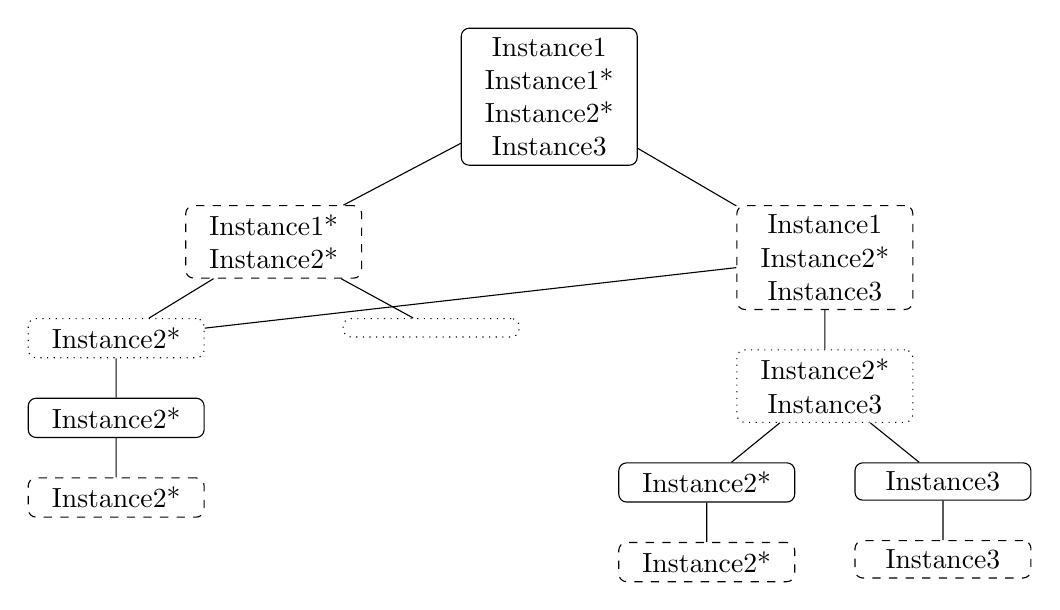
\begin{tikzpicture}[
    reaction/.style={rectangle, draw, rounded corners=1mm, text width=2cm,
        text centered, anchor=north},
    activation/.style={rectangle, draw, rounded corners=1mm, dashed, text width=2cm,
        text centered, anchor=north},
    push/.style={rectangle, draw, rounded corners=1mm, dotted, text width=2cm,
        text centered, anchor=north},
    level 1/.style={sibling distance=7.0cm},
    level 2/.style={sibling distance=4.0cm},
    level 3/.style={sibling distance=3.0cm},
    level distance=0.5cm, growth parent anchor=south
]
\node (Action) [reaction] {Instance1 Instance1* Instance2* Instance3}
  child {
    node (Activation01) [activation] {Instance1* Instance2*}
    child {
      node (Push01) [push] {Instance2*}
      child {
        node (Reaction01) [reaction] {Instance2*}
        child {
          node (Activation03) [activation] {Instance2*}
        }
      }
    }
    child {
      node (Push02) [push] {}
    }
  }
  child {
    node (Activation02) [activation] {Instance1 Instance2* Instance3}
    child {
      node (Push03) [push] {Instance2* Instance3}
      child {
        node (Reaction02) [reaction] {Instance2*}
        child {
          node (Activation04) [activation] {Instance2*}
        }
      }
      child {
        node (Reaction03) [reaction] {Instance3}
        child {
          node (Activation05) [activation] {Instance3}
        }
      }
    }
  }
;

\draw (Activation02) -- (Push01);

\end{tikzpicture}
\endgroup
%%}%
\caption{Example mutable phase access set calculation\label{access_sets}}
\end{figure}

Figure~\ref{access_sets} shows the mutable phase access set calculation for the transaction illustrated in Figure~\ref{transaction}.
The root shows that Instance1 does not change in at least one activation (Instance1) and may change in at least one activation (Instance1*), that Instance2 may change in every activation (Instance2*), and that Instance3 is read-only in this transaction (Instance3).
The empty node in Figure~\ref{access_sets} comes from an unbound push port.

The second step for detecting a non-deterministic transaction is to verify that a mutated instance appears in at most one child node access set for the activation and push port nodes.
Let $\mathit{race}: \{ H \} \times \{ H \} \to \mathcal{B}$ be a predicate that indicates a data race between two access sets.
This function is defined as follows:
\begin{multline}
  \mathit{race} (H_1, H_2) = \\
  (\exists i : (i, \mathit{Write}) \in H_1 \land (i, x) \in H_2) \lor
  (\exists j : (j, \mathit{Write}) \in H_2 \land (j, y) \in H_1)
\end{multline}
This is, a component that changes state in one access set may not appear in the other access set.
The $\mathit{race}$ predicate is computed for each pair of child mutable phase access sets in activation and push port nodes.
This check succeeds everywhere but Activation2 in Figures~\ref{transaction}~and~\ref{access_sets}, as Instance2* appears in both children.
The activation and push port nodes represent activities that will be performed together.
That is, once control passes to an activate statement, all push ports and their bound reactions are activated.
In contrast, activations (as children of action and reaction nodes) represent mutually exclusive alternatives:  at most one activate statement is executed per action/reaction body.
Thus, a mutated instance appearing in two or more children of an activation node or push port node indicates that the state of a component may be mutated in disparate ways leading to a non-deterministic transaction.

\paragraph{Complexity.}
Maintaining appropriate forward and reverse hash maps of the bindings allows the binding check to be performed in $O(N)$ time where $N$ is the number of ports in the system.
Similarly, the construction of a transaction graph can be performed in $O(|N| + |V|)$ time where $|N|$ is the number of nodes in the transaction and $|V|$ is the number of edges.
Proving that a transaction is acyclic can be performed in $O(|N| + |V|)$ time where $|N|$ is the number of nodes and $|V|$ is the number of edges.

A loose upper-bound on the complexity of the access set calculations for the non-determinism check is $O(k |N|^2 \log (|N|))$ where $|N|$ represents the number of nodes in a transaction and $k$ represents the maximum branching factor in the transaction.
The size of the access set for the root is $|N|$.
Assuming a naive set implementation, the complexity of computing the access set for the root is $O(|N| \log (|N|))$.
This must be repeated $k$ times for all nodes in the graph resulting in an overall complexity of $O(k |N|^2 \log (|N|))$.

A loose upper-bound on the complexity of the compatibility check is also $O(k |N|^2 \log (|N|))$.
Assume that the size of the access set at each node is $|N|$.
A tree-based set lookup can be performed in $O(\log(|N|))$ time.
The lookup must be performed $k |N|$ times by the parent.
The lookup must repeated for each of the $|N|$ nodes for a combined complexity of $O(k |N|^2 \log (|N|))$.

The complexity of these algorithms has not presented a problem in practice as most of the systems we have implemented have small numbers for $|N|$, $|V|$, and $k$.

\section{Activations}
\label{activations}

When executing a transaction, the \rcgo{} run-time system must execute the immutable phase of all implied state transitions before executing any of the mutable phases.
To accomplish this, the run-time system uses a novel calling convention to create a list of deferred contexts and statements that represent the mutable phase of each state transition.
The immutable phase constructs the list and the mutable phase processes the list.
To present the calling convention, we first present some details about the run-time system such as the ordinary calling convention and push ports.
We then describe the behavior of the calling convention and explain it using an illustrative example.

\paragraph{Ordinary calling convention.}
The ordinary call mechanism in the \rcgo{} run-time system is similar to the C-decl calling convention.
It assumes the existence of an \emph{instruction pointer}, which contains the address of the currently executing instruction, and a \emph{base pointer} that points to a location in the stack, which can be offset to access arguments and local variables.
An ordinary call in the language is accomplished through the following sequence:
\begin{enumerate}
\item (Caller) Create space for return values.
\item (Caller) Push arguments onto the stack, left to right.
\item (Caller) Push the instruction pointer onto the stack and transfer control to the body of the function, method, action, reaction, getter, or initializer.
\item (Callee) Push the base pointer onto the stack and set the base pointer to the top of the stack.
\item (Callee) Reserve space on the stack for local variables.
\item (Callee) Execute the body of the function, method, etc.
\item (Callee) Pop the local variables, pop and restore the base pointer, pop and restore the instruction pointer.
\item (Caller) Pop the arguments.
\item (Caller) Pop the return values.
\end{enumerate}
The major difference between this calling convention and C-decl is that the arguments are pushed in the opposite order to match the semantics of Go.
The collection of arguments, previous instruction pointer, previous base pointer, and reserved space is called a \emph{stack frame} (or \emph{call frame}).
Figure~\ref{frame} shows the layout of a normal stack frame.
For this presentation, we assume that the stack grows down, i.e., the previous base pointer has a lower address in memory than the previous instruction pointer.

\begin{figure}
\centering
\resizebox{.5\textwidth}{!}{%
\begingroup
\fontsize{10pt}{12pt}\selectfont
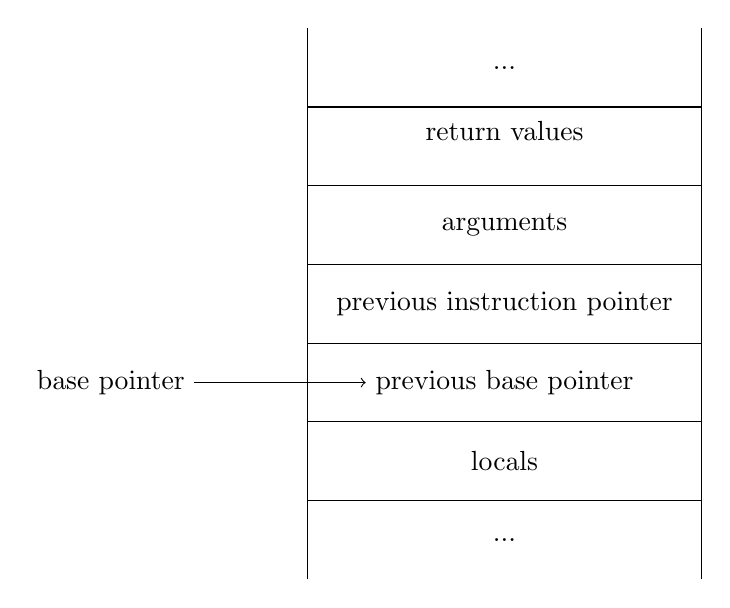
\begin{tikzpicture}
%% component boundary

\draw (0,1) -- (0,8);
\draw (5,1) -- (5,8);

\node at (2.5, 7.5) { ... };
\draw (0,7) -- (5, 7);
\node at (2.5, 6.7) { return values };
\draw (0,6) -- (5,6);
\node at (2.5, 5.5) { arguments };
\draw (0,5) -- (5,5);
\node at (2.5, 4.5) { previous instruction pointer };
\draw (0,4) -- (5,4);
\node (pbp) at (2.5, 3.5) { previous base pointer };
\draw (0,3) -- (5,3);
\node at (2.5, 2.5) { locals };
\draw (0,2) -- (5,2);
\node at (2.5, 1.5) { ... };

\node (bp) at (-2.5, 3.5) { base pointer };
\draw[->] (bp) -- (pbp);

\end{tikzpicture}
\endgroup
}%
\caption[Diagram of a stack frame]{Diagram of a stack frame.  The stack is depicted as growing down.}
\label{frame}
\end{figure}

\paragraph{Push ports.}
A push port is a field in a component, which is implemented as a pointer to a linked list that contains the component pointer/reaction pairs that are bound to the push port.
The \rcgo{} run-time system populates each push port before execution begins.

\paragraph{Synchronized two-phase calling convention.}
As was previously stated, the execution of an activate statement is split into an immutable phase and a mutable phase.
To prepare for the mutable phase, the immutable phase must preserve the stack frame (context) of the action or reaction that executes an activate statement and must record which activate statement was executed so that the same activation can be resumed in the mutable phase.
To accomplish this, we devised the \emph{synchronized two-phase calling convention}, which is used to execute activate statements during the immutable phase.

Recall that activate statements may only appear in actions and reactions.
After executing the immutable phase of an activate statement in a reaction, control must be returned to the calling activate statement so that it may activate other push ports.
After executing the immutable phase of an activate statement in an action, control must be returned to the \rcgo{} run-time system to begin the mutable phase.

In the ordinary calling convention, the stack frame for the reaction would be popped, control would be returned to the caller, and the arguments would be popped.
To preserve the stack frame for use during the mutable phase, however, the activate statement returns control to the caller without popping the frame and the caller does not pop the arguments.
Thus, the complete frame for the reaction is preserved on the stack.

Each such deferred stack frame is added to a list to make it available in the mutable phase.
Let $head$ be a variable containing a pointer, initially nil, which will serve as the head of a linked list.
Before the activate statement returns from the immutable phase, it sets the previous base pointer in the deferred stack frame to the value of $head$ and updates head to be the current base pointer which inserts the stack frame into the list.
The \rcgo{} run-time system can iterate over the elements of the list by following the previous base pointer to access all of the stack frames that are needed for the mutable phase.
If the list is empty ($head$ is nil), then no activate statement was executed and the mutable phase may be skipped.

The final piece of information that must be recorded is the body of the activate statement so that it is accessible in the mutable phase.
Before returning from the immutable phase, the activate statement records the body of the activate statement in the previous instruction pointer slot of the current stack frame.
It is safe to use the previous instruction pointer because it is not used beyond the immediate return.
Furthermore, it is at a fixed location, which allows it to be accessed in any deferred stack frame.

The synchronized two-phase calling convention is used when executing an activate statement and proceeds as follows:
\begin{enumerate}
\item Save the previous base pointer of the current stack frame in $bp$.
\item Set the previous base pointer of the current stack frame to the value of $head$.
\item Set $head$ to the value of the base pointer.
\item Save the previous instruction pointer of the current stack frame in $ip$.
\item Set the previous instruction pointer of the current stack frame to the body of the activate statement.
\item For each push port in the port call list:
  \begin{enumerate}
  \item Push the arguments to the push port onto the stack.\label{step1}
  \item For each component pointer/reaction pair in the push port:
    \begin{enumerate}
    \item Push the component pointer onto the stack.
    \item Copy the arguments prepared in~\ref{step1} onto the stack.
    \item Call the reaction.
    \end{enumerate}
  \end{enumerate}
\item Set the base pointer to the value of $bp$ and return control to the address in $ip$.
\end{enumerate}

The synchronized two-phase calling convention evaluates the arguments to a push port once and passes a copy to each bound reaction.
An alternative would be to evaluate the arguments for each bound reaction.
This means that the arguments may not be evaluated (i.e., the push port is not bound to any reactions) or may be evaluated multiple times.
If the arguments contain an expression with side-effects, then the behavior of the code becomes dependent on composition.
While this may be desirable in some cases, we opted for making a port call resemble an ordinary function call as much as possible.
This sentiment also influenced our decision to pass a copy of the arguments to each reaction as opposed to reusing the same set of prepared arguments.
Since each reaction starts with a copy of the arguments, it is free to manipulate them as allowed by the semantics of Go.
Furthermore, the arguments are available in the mutable phase which obviates the need to make local copies of arguments.
This approach assumes that copying arguments does not generate significant overhead.

%% After an activate statement calls the last push port, it makes temporary copies of the instruction pointer and base pointer of the caller.
%% It may then safely overwrite the base pointer to insert itself into the list of mutable phase stack frames and it may safely overwrite the instruction pointer with the body of the activate statement.

A major caveat when using the synchronized two-phase calling convention is that it must be assumed that the stack pointer changes when calling a push port.
To illustrate why this is an issue, consider the case when a caller wishes to preserve the contents of a register.
One strategy is to push the contents of the register onto the stack, perform the call, and then pop the value from the stack into the register.
After calling a push port, the caller may no longer assume that the previous value of the register is at the top of the stack.
An easy work-around is to allocate local variables, i.e., variables whose addresses are relative to the base pointer instead of the stack pointer, for saving temporary values that must persist across a push port call.
In the same way, the variables used to iterate over the list of component/reaction pairs in a push port should be allocated as local variables so that they may survive the calls to the reactions.

\paragraph{Mutable phase.}
The mutable phase consists of executing all of the deferred activate statements.
The algorithm for doing so is as follows:
\begin{enumerate}
\item If the value of $head$ is nil, stop.  Otherwise, set the base pointer to the value in $head$.
\item Transfer control to the instruction indicated by the previous instruction pointer\label{transfer}.  Execution continues until the body of the activate statement (implicitly or explicitly) returns.
\item If the previous base pointer is nil, stop.  Otherwise, set the base pointer to the previous base pointer and go to \ref{transfer}.
\end{enumerate}

The algorithm iterates over the list of deferred stack frames accessible through $head$.
The last element in the list is indicated by a previous base pointer that is nil.
Control is transferred to the previous instruction pointer which contains the body of the activate statement.

\begin{figure}
\centering
\resizebox{.75\textwidth}{!}{%
\begingroup
\fontsize{10pt}{12pt}\selectfont
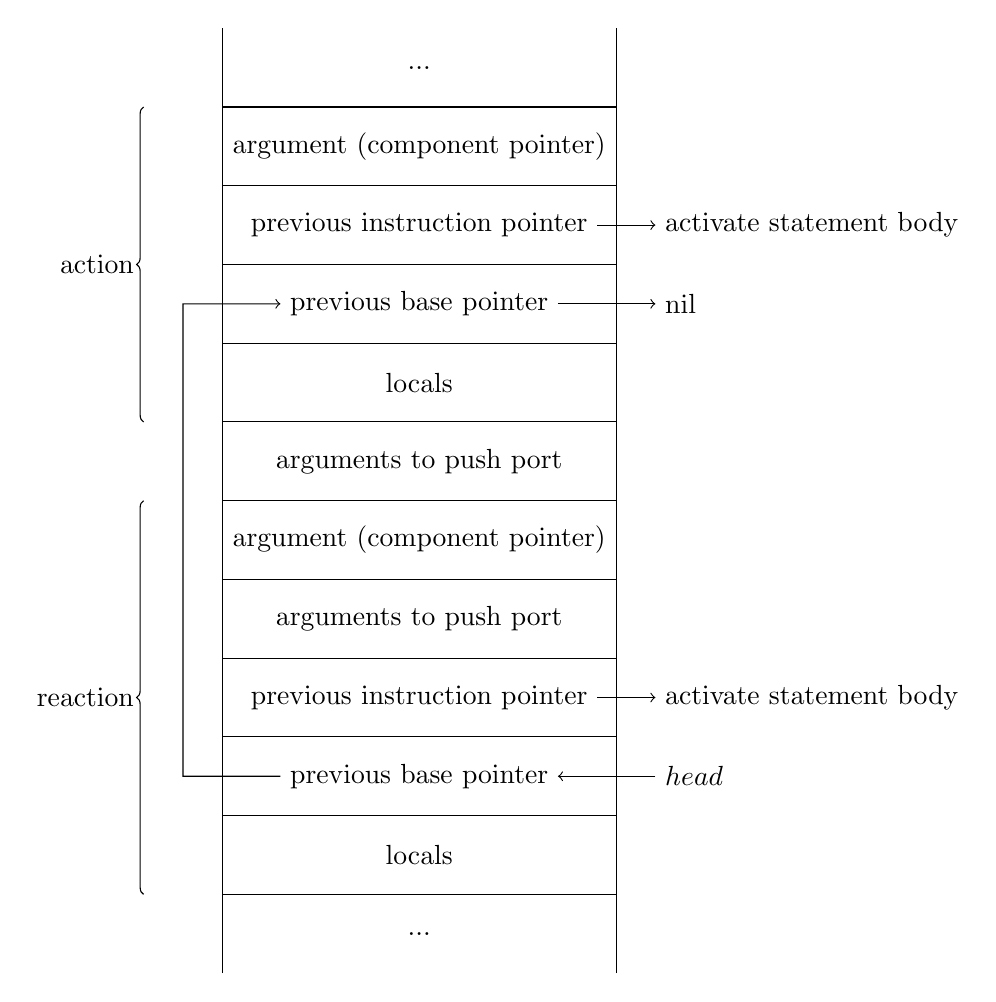
\begin{tikzpicture}
%% component boundary

\draw (0,-5) -- (0,7);
\draw (5,-5) -- (5,7);

\node at (2.5, 6.5) { ... };
\draw (0,6) -- (5,6);
\node at (2.5, 5.5) { argument (component pointer) };
\draw (0,5) -- (5,5);
\node (pip1) at (2.5, 4.5) { previous instruction pointer };
\draw (0,4) -- (5,4);
\node (pbp1) at (2.5, 3.5) { previous base pointer };
\draw (0,3) -- (5,3);
\node at (2.5, 2.5) { locals };
\draw (0,2) -- (5,2);
\node at (2.5, 1.5) { arguments to push port };
\draw (0,1) -- (5,1);
\node at (2.5, .5) { argument (component pointer) };
\draw (0,0) -- (5,0);
\node at (2.5, -.5) { arguments to push port };
\draw (0,-1) -- (5,-1);
\node (pip2) at (2.5, -1.5) { previous instruction pointer };
\draw (0,-2) -- (5,-2);
\node (pbp2) at (2.5, -2.5) { previous base pointer };
\draw (0,-3) -- (5,-3);
\node at (2.5, -3.5) { locals };
\draw (0,-4) -- (5,-4);
\node at (2.5, -4.5) { ... };

\node[anchor=west] (as1) at (5.5, 4.5) { activate statement body };
\draw[->] (pip1) -- (as1);
\node[anchor=west] (as2) at (5.5, -1.5) { activate statement body };
\draw[->] (pip2) -- (as2);

\draw[->] (pbp2) -- ++(-3,0) -- ++(0,6) -- (pbp1);

\node[anchor=west] (nil) at (5.5, 3.5) { nil };
\draw[->] (pbp1) -- (nil);

\node[anchor=west] (head) at (5.5, -2.5) { $head$ };
\draw[->] (head) -- (pbp2);

\draw[decorate,decoration={brace}] (-1,2) -- (-1,6) node[anchor=east,midway] { action };

\draw[decorate,decoration={brace}] (-1,-4) -- (-1,1) node[anchor=east,midway] { reaction };

\end{tikzpicture}
\endgroup
}%
\caption[Diagram of the stack after the immutable phase for single action-reaction]{Diagram of the stack after the immutable phase when an action activates a single reaction}
\label{activation_ex_1}
\end{figure}

\paragraph{Example:  one action, one reaction.}
Suppose an action activates a single push port that is bound to a single reaction and the reaction has a single activation that does not activate any push ports.
Figure~\ref{activation_ex_1} shows a diagram of the stack after the immutable phase for this scenario.
The stack contains two frames, one corresponding to the action and one corresponding to the reaction.
The $head$ variable points to the reaction frame which in turn points to the action frame using the previous base pointer slot.
The action frame points to nil indicating that it is the last frame in the list.
The previous instruction pointers point to the bodies of the activate statements.
Between the frames are the push port arguments which are duplicated for the call to the reaction.
If the push port had been bound to multiple reactions, then the reaction portion of the diagram would be replicated to match the number of bound reactions.
If multiple push ports were activated by the activate statement, then additional push port arguments and reactions would appear on the stack.

\paragraph{Calling convention efficiency.}
The synchronized two-phase calling convention has the potential to be as efficient as a function or method call.
The proposed calling convention can be implemented directly on modern hardware architectures like x86 and x86\_64, which contain all of the registers and instructions necessary to support the synchronized two-phase calling convention.
The synchronized two-phase calling convention relies solely on the stack which means that the underlying operating system must set up the stack, back it with memory pages, etc.
More importantly, it avoids the overhead of heap allocation.
Port calls resemble virtual method calls in that the reactions may need to be looked up before they can be executed.
However, this lookup could be avoided by inlining the body of each reaction using the substitutional equivalence property.
This could be performed prior to execution or during execution using just-in-time compilation techniques.
We leave the application of these techniques to future work.

\section{Heaps}
\label{heaps}

In this section, we describe the implementation of the heap data type introduced in Chapter~\ref{language} and our approach to garbage collection.
Our approach to implementing dynamic memory allocation and garbage collection was shaped by the independence of state required by the semantics of reactive components.
Thus, instead of relying on a single global heap, the implementation contains a heap for each component that can be garbage collected independently of the others.
This independence allows garbage collection to be performed concurrently with other activities using simple, single-threaded algorithms.

\paragraph{Slots and blocks.}
A \emph{slot} is the smallest unit of memory that can be dynamically allocated.
Typically, a slot is the size of two pointers.
A \emph{block} is an extent of memory and a set of bits indicating the allocation status of each slot in the extent.
The status bits indicate if a slot is allocated, if a slot is the beginning of an object, and if the slot has been marked by the mark-and-sweep algorithm.
Blocks also contain left and right pointers that allow them to be formed into a binary tree ordered by the address of the extent.

\paragraph{Mark-and-sweep garbage collection.}
We implemented a simple mark-and-sweep algorithm to collect garbage in a tree of blocks.
The core of the marking phase involves scanning extents for pointers to objects.
When the algorithm comes across a slot that is allocated, marked, and which contains a pointer-sized value that points to a location in the tree of blocks that is also allocated, it marks the object indicated by the pointer.
The algorithm is bootstrapped by marking all slots in a designated root object.
The algorithm repeatedly scans the extents in the tree of blocks until no new marks can be added.
At this point, the sweep phase resets the allocated bit for all slots that are allocated but not marked and resets the marked bit for the next run of the algorithm.
A block that is not marked, meaning that none of its slots were marked, is removed from the tree of blocks and deallocated.

\paragraph{Heaps.}
A \emph{heap} contains a root block, a list of unallocated chunks of memory (free list), and pointers to create a tree structure.
When allocating an object from a heap, the heap attempts to find an adequate chunk in the free list using a first-fit policy.
If this fails, the heap allocates a new block, inserts it into the tree and free list, and then allocates again using the newly inserted chunk.
The sweep phase of the mark-and-sweep algorithm reconstructs the free list.

As described in Chapter~\ref{language}, every component has an associated heap.
A heap of this kind is called an \emph{implicit heap}.
Heaps that are created via \verb+new+ and passed to \verb+move+, \verb+merge+, and \verb+change+ are called \emph{explicit heaps}.
All heaps have a distinguished root object.
The marking phase of the mark-and-sweep algorithm is seeded with this root object.
The root object of an implicit heap contains the statically allocated state of the component that owns the heap.
The root object of an explicit heap is an object that is allocated in the same heap.

The semantics of reactive components allow heaps to form strict hierarchies, i.e., a tree structure where the root of the tree is an implicit heap and the internal nodes and leaves of the tree are explicit heaps.
A strict hierarchy gives a graphical interpretation to merge and move operations.
A move operation moves a sub-tree from one location to another location.
 Merging a heap $h$ into another heap $p$ involves removing $h$ from the tree, inserting the blocks of $h$ into the tree of blocks of $p$, merging the free list of $h$ into the free list of $p$, and inserting the children of $h$ as children of $p$.

\paragraph{The active heap.}
Logically, the \rcgo{} run-time system maintains a stack of heaps where the top of the stack represents the \emph{active heap}.
The active heap is used to satisfy all dynamic memory requests, i.e., calls to \verb+new+.
The implicit heap that is associated with the receiving component is pushed/popped upon entering/leaving an action, reaction, getter, or initializer.
Specific \verb+change+ statements are used to push and pop explicit heaps.
Thus, the call stack (i.e., the \verb+change+ statements that are active on the call stack) implements the stack of heaps.
When a new heap is created, it is inserted as a child of the active heap.

\paragraph{Atomicity.}
Chapter~\ref{language} describes how the semantics of reactive components permit concurrent access to heaps.
The first scenario where this may occur is when a heap is passed to a push port that is bound to multiple reactions.
The semantics of reactive components allow the reactions to be executed concurrently.
Thus, two different threads may attempt to move/merge the same heap at the same time.
The second scenario occurs when a component is concurrently accessed in multiple transactions that don't mutate the state of the component.
The action, reaction, or getter is allowed to allocate memory, which means that heaps must correctly handle concurrent access.
Our implementation of heaps uses the Thread Safe Interface pattern~\cite{schmidt2000pattern} to synchronize access to heaps when allocating, moving, and merging.

\paragraph{Heap links.}
Heaps are exposed to users via pointers to heaps, e.g., \verb+*heap int+.
These pointers to heaps can be stored in objects allocated in another heap.
The semantics of \verb+change+, \verb+merge+, and \verb+move+ ensure that the parent-child relationships formed by pointers to heaps match exactly those known by the run-time system.
The two rules that enforce this behavior are that 1) \verb+merge+ and \verb+move+ fail for any heap that is already on the stack of active heaps and 2) all pointers in scope become foreign in the body of a change statement.
The second rule forces the user to \verb+move+ heaps if they desire to change the hierarchy, because pointers with foreign indirection mutability cannot be stored.
Recall that the stack of active heaps is set up by active \verb+change+ statements.
Using the inductive argument that the parent-child relationship was previously correct, then the ancestors of the active heap must all appear in the stack of active heaps.
Thus, failing to \verb+merge+ and \verb+move+ heaps on the active stack prevents the formation of cycles.

\begin{figure}
\centering
%%\resizebox{\textwidth}{!}{%
\begingroup
\fontsize{10pt}{12pt}\selectfont
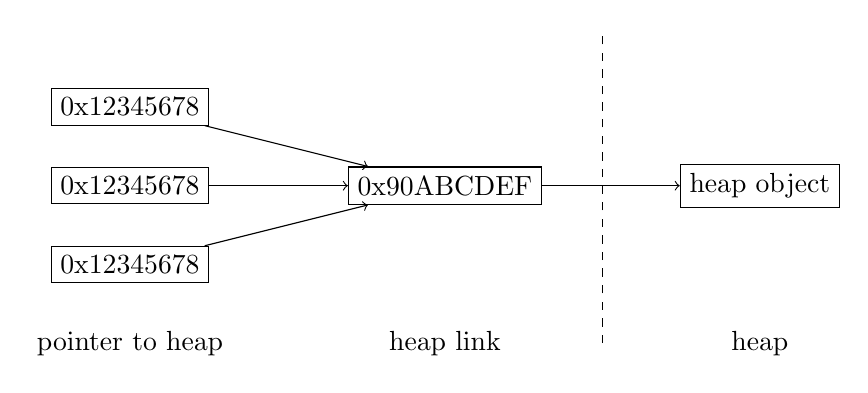
\begin{tikzpicture}
\node [rectangle, draw] (p1) at (0,1) {0x12345678};
\node [rectangle, draw] (p2) at (0,0) {0x12345678};
\node [rectangle, draw] (p3) at (0,-1) {0x12345678};
\node at (0,-2) {pointer to heap};
\node [rectangle, draw] (hl) at (4,0) {0x90ABCDEF};
\node at (4,-2) {heap link};
\node [rectangle, draw] (heap) at (8,0) {heap object};
\node at (8,-2) {heap};
\draw [->] (p1) -- (hl);
\draw [->] (p2) -- (hl);
\draw [->] (p3) -- (hl);
\draw [->] (hl) -- (heap);
\draw [dashed] (6, -2) -- (6, 2);
\end{tikzpicture}
\endgroup
%%}%
\cprotect\caption[Heap link example]{Example illustrating heap links.  The objects on the far left represent user-level pointers to heaps, e.g., \verb+* heap int+.  The middle object is a heap link, which contains the address of the child heap that appears on the far right.}
\label{heap_link}
\end{figure}

As illustrated in Figure~\ref{heap_link}, a user-level pointer to a heap points to an object called a heap link which in turn points to a heap.
The objects on the left side of the diagram are objects in the parent heap and the object on the right is the child heap.
The extra level of indirection introduced by the heap link concentrates all references to the child heap into one location.
Moving a heap involves reading the pointer out of the heap link and replacing it with \verb+nil+.
This makes the heap inaccessible to the previous owner (parent), which maintains the isolation of state between reactive components.
The marking phase of the mark-and-sweep algorithm is aware of heap links and marks heaps as being reachable from another heap.
Unreachable heaps are pruned from the hierarchy during garbage collection.

\paragraph{Concurrent garbage collection.}
Two features of reactive components permit concurrent garbage collection.
First, the state of each reactive component is isolated which allows garbage collection to be performed on different components at the same time without conflict.
Second, garbage collection can be framed as an action to be executed by the scheduler.
Thus, associated with each component is an action that invokes the garbage collector on the implicit and explicit heaps of the corresponding component.
Furthermore, the action is considered to modify the state of the component which prevents all transactions involving the component from executing concurrently with the garbage collection action.
We assume that the scheduler executes the garbage collection action often enough that no additional invocations of the garbage collector are necessary.
More plainly, we do not trigger the garbage collector in the allocation routine, which is the approach taken by many systems using garbage collection.
Most garbage collection algorithms include a scan of the call stack as objects reachable from the call stack must not be collected.
In our approach, such scanning is useless since the call stack is empty when executing the garbage collection action and the root object is embedded in the implicit heap that is being collected.

\section{I/O}

A possible bottom-up approach to support reactive components would be to write a kernel for reactive components, i.e., a scheduler and memory manager, and then write an operating system and application suites using reactive components.
This approach, however, is impractical and risky given the expense of developing software for an as yet unproven technology.
A top-down approach instead involves proving the utility of reactive components at the application layer and then proceeding to lower layers when appropriate.
This approach far less risky and is the one taken in this chapter.
To develop and evaluate real-world applications, the input/output facilities of the host operating system then must be exposed to reactive components so that they may communicate and interact with other processes and systems.
This section describes our approach to exposing the input/output (I/O) facilities of a Linux/GNU system to reactive components.

A Linux/GNU system offers a variety of I/O and communication mechanisms including pipes, sockets, shared memory, and message queues.
For our purposes, we focused on mechanisms that are available through a file descriptor interface.
Our approach consists of two steps.
The first step is to add file descriptors and operations for manipulating them, such as read and write, to the \rcgo{} language.
The second step was to wrap file descriptors in reactive components to make their functionality available via a conventional reactive component interface.

The main consideration when supporting file descriptors was to ensure that reads and writes were non-blocking, as a blocking read or write may violate fairness.
A transaction that blocks on a read or write would adversely affect the latency and throughput of the scheduler as the scheduler thread would be blocked and not able to service other transactions.
Furthermore, a blocking transaction holds the locks for all components involved in that transaction, and other enabled transactions that also involve those components would be denied service which also violates the fairness requirement of the scheduler.
To prevent these problems, all file descriptors when they are created are set to be non-blocking.
Thus, all subsequent reads and writes are also non-blocking.

Threaded programs using non-blocking I/O typically use some kind of synchronous I/O multiplexing which allows a thread to determine which file descriptors are ready for reading and/or writing.
The goal in doing so is to allow a thread to service multiple file descriptors and yield the processor if no file descriptors are ready.
To map this concept into reactive components, we introduced a \verb+readable+ function that tests if a file descriptor is ready for reading and a \verb+writable+ function that tests if a file descriptor is ready for writing.
These functions are intended to be used in preconditions so that an action becomes enabled when the corresponding file descriptor is ready.

The \verb+readable+ and \verb+writable+ functions are also used as part of the termination protocol of the Partitioned scheduler described in Section~\ref{scheduler_implementation}.
When the termination protocol enters the checking phase where it attempts to prove that every precondition is false, it records which file descriptors are being checking for readability and writability.
If the termination protocol proves that all preconditions are false but some preconditions depend on readability or writability, it enters a state where it waits for one of the file descriptors to become ready.
This allows a system of reactive components to sleep while it waits for external input like a message from a remote host or a timer.

Conceptually, a file descriptor contains component state and should be subject to all of the constraints of normal component state.
The two main constraints are 1) it cannot be shared by another component and 2) it cannot change in the immutable phase of a transaction.
To enforce the first constraint, file descriptors are implemented as dynamically allocated opaque data structures.
Forcing dynamic allocation makes file descriptors subject to the pointer sharing rules, i.e., they can only be shared via foreign indirection mutability in the immutable phase.
Making the data structure opaque prevents sharing through copying.
The normal immutable phase rules in concert with properly declared built-in functions prevent file descriptors from changing in the immutable phase.
That is, functions like \verb+read+ and \verb+write+ require a pointer to a file descriptor with mutable indirection mutability.

To test these ideas, we implemented a Simple Network Time Protocol (SNTP) client.
SNTP attempts to acquire the current time from a server while simultaneously measuring a round-trip latency to determine an accurate local time.
The client timestamps the request with the local time and sends it to the server.
The server timestamps the request when it arrives and again when it sends it back to the client.
Finally, the client timestamps the request when it receives it back from server.
The client uses the timestamps to determine the offset of the local clock from the clock on the server.
This procedure is repeated periodically to synchronize the local clock.
The messages are exchanged using the User Datagram Protocol (UDP).

\begin{figure}
\centering
\resizebox{\textwidth}{!}{%
\begingroup
\fontsize{10pt}{12pt}\selectfont
\begin{tikzpicture}
\draw (2,7.5) rectangle (4,9);
\node[below] at (3,9) {Timer};
\rapush[4,8,1.8,.5,alarma,ignore]{Alarm()};

\draw (1.5,6) rectangle (16.5,10);
\node[below] at (8.5,10) {Sntp};
\lppush[5,8,1.8,.5,alarmb,ignore]{Alarm()};
\rapush[11,8,3.5,.5,senda,ignore]{Send(UdpMessage)};
\rppush[11,7,4.1,.5,receivea,ignore]{Receive(UdpMessage)};

\draw (12,6.5) rectangle (16,9);
\node[below] at (14,9) {UdpParticipant};
\lppush[12,8,3.7,.5,sendb,ignore]{Send(UdpMessage)};
\lapush[12,7,3.8,.5,receiveb,ignore]{Receive(UdpMessage)};

\draw (alarma.center) -- (alarmb.center);
\draw (senda.center) -- (sendb.center);
\draw (receivea.center) -- (receiveb.center);

\end{tikzpicture}
\endgroup
}%
\caption{Diagram of a Simple Network Time Protocol (SNTP) client\label{sntp}}
\end{figure}

Figure~\ref{sntp} shows a diagram of the SNTP client application.
The top-level Sntp component contains two sub-components:  Timer and UdpParticipant.
The Timer component is a periodic timer implemented by wrapping a \verb+timerfd+ file descriptor.
The UdpParticipant component wraps a UDP socket file descriptor and is capable of sending and receiving UDP messages.
The Sntp component uses these components to implement an SNTP client.
Whenever the Timer fires the alarm, the UdpParticipant creates an SNTP request and sends it using the UdpParticipant.
This all happens as part of one atomic transaction.
Whenever the UdpParticipant receives a message, it passes it to the Sntp component which deserializes it, timestamps it, and interprets it to compute the local clock offset.

The Sntp component demonstrates how composition (with reactive components for I/O) can be used to construct systems.
The Timer and UdpParticipant components are generic since they do not contain any SNTP related logic.
Furthermore, they have well-defined concurrency semantics that will be enforced when they are composed in other systems.
Thus, it is possible to use the reactive component model to produce reusable \emph{reactive} software.

\section{Summary}

The goal of implementing reactive components was to test the practicality of the reactive component model.
Specifically, we desired to know how the various features of the model could be implemented, which features were troublesome, and how the implementation utilizes various assumptions.
Flexibility in the reactive component model necessitates a check for sound composition.
The sound composition algorithm described in Section~\ref{sound_composition} uses the static system assumption and the component proxy assumption to generate a graphical model of each transition and check it for determinism.
A cursory analysis yielded an upper bound of $O(k n^2 \log (n))$ where $n$ is the number of instances involved in the transaction and $k$ is the maximum branching factor in the transaction.

To implement activate statements, we developed the synchronized two-phase calling convention which executes the immutable phase of a transaction first and preserves the context necessary for the second (mutable) phase.
The synchronized two-phase calling convention was implemented using standard function call and stack manipulation facilities.

The isolation of component state is enforced in two ways.
First, the type system prevents components from sharing pointers directly via \verb+$const+ and \verb+$foreign+ modifiers.
Second, the implementation uses garbage collection to prevent indirect sharing through dangling pointers.
In this chapter, we describe the implementation of heaps and how they are used for dynamic memory allocation.
Heaps are designed so that they can be merged and moved.
At the user level, all references to a heap are encapsulated by a ``link'' which is used to enforce atomic moves and merges.
The independence of state between components allows each component to have its own heap (or tree of heaps) that can be garbage collected independently of other components.
Garbage collection can be conducted in parallel by associating a garbage collection action with each component.

To enhance the practicality of the reactive component implementation, we introduced file descriptor I/O that allows reactive components to interact with a variety of operating system facilities.
All I/O is non-blocking to preserve the fairness of the scheduler.
Components may use the \verb+readable+ and \verb+writable+ functions to test file descriptors.
The scheduler uses these functions as part of the termination protocol to sleep while waiting for external inputs.
File descriptors are treated as component state and therefore cannot be shared between components or mutated during the immutable phase.
Using file descriptor I/O, we implemented an SNTP client, which demonstrates how systems can be built up from simple components.
